\documentclass[tikz]{standalone}
\usepackage[utf8]{inputenc}
\usepackage[T1]{fontenc}
\usepackage{ifthen} 

\usepackage{../../templates/moeptikz}
\usepackage[utf8]{inputenc}
\usepackage[T1]{fontenc}

\usepackage{circledsteps}

\RequirePackage{xcolor}

%% HPI color definitions according to the design manual
% These do not exactly match the RGB values used in the Powerpoint slide master due to unknown reasons
\definecolor{hpiyellow}{RGB}{246,168,0}
\definecolor{hpiorange}{RGB}{221,97,8}
\definecolor{hpired}{RGB}{177,6,58}
\definecolor{hpigray}{RGB}{90,96,101}
\definecolor{hpiblue}{RGB}{0,122,158}


\renewcommand{\sfdefault}{neosans}
% Different font weights for neosans
\newcommand{\textl}[1]{{\fontseries{l}\selectfont #1}} % light
\newcommand{\textm}[1]{{\fontseries{m}\selectfont #1}} % medium, same as default weight
\newcommand{\textsb}[1]{{\fontseries{sb}\selectfont #1}} % semibold
\newcommand{\textmb}[1]{{\fontseries{mb}\selectfont #1}} % bold, same as \textbf
\newcommand{\texteb}[1]{{\fontseries{eb}\selectfont #1}} % extra bold
\newcommand{\textub}[1]{{\fontseries{ub}\selectfont #1}} % ultra bold

\tikzset{every picture/.style={/utils/exec={\sffamily}}}
\tikzset{flipflop RSflanke/.style={
  flipflop,
  flipflop def={t1=S, t2=C, c2=1, t3=R, t6=Q, t4={\ctikztextnot{Q}}}
}}


\tikzset{
  mechanicalSwitch/.pic={
    \coordinate (-inUp) at (135:2); 
    \coordinate (-inDown) at (235:2);
    \coordinate (-out) at (2,0);
    \coordinate (-center) at (0,0);
    
    \draw (0,0) circle [radius = 2cm];
    \draw [fill=gray!20] (0,0) circle [radius = 0.2cm];

    \draw (0, 0) -- (2, 0);
    \draw (135:.8) -- (135:2); 
    \draw (225:.8) -- (225:2); 

    \draw [fill=gray!20] (2, 0) circle [radius=0.05cm]; 
    \draw [fill=gray!20] (135:2) circle [radius=0.05cm]; 
    \draw [fill=gray!20] (225:2) circle [radius=0.05cm]; 

    
    \draw [thick] (0,0) -- (175:1.5); 

    \draw [dashed, <->, domain=135:225] plot ({cos(\x)}, {sin(\x)}); 
  },
  mechanicalSwitchClosed/.pic={
    \coordinate (-inUp) at (135:2); 
    \coordinate (-inDown) at (255:2);
    \coordinate (-out) at (2,0);
    \coordinate (-center) at (0,0);
    \draw (0,0) circle [radius = 2cm];
    \draw [fill=gray!20] (0,0) circle [radius = 0.2cm];

    \draw (0, 0) -- (2, 0);
    \draw (135:.8) -- (135:2); 
    \draw (225:.8) -- (225:2); 

    \draw [fill=gray!20] (2, 0) circle [radius=0.05cm]; 
    \draw [fill=gray!20] (135:2) circle [radius=0.05cm]; 
    \draw [fill=gray!20] (225:2) circle [radius=0.05cm]; 

    
    \draw [thick] (0,0) -- (135:2); 

    \draw [dashed, <->, domain=135:225] plot ({cos(\x)}, {sin(\x)}); 
  }
}


\usetikzlibrary{calc}
\usetikzlibrary{positioning}


\usetikzlibrary{positioning,decorations.pathreplacing, calc, shapes.multipart, ext.positioning-plus}



\begin{document}

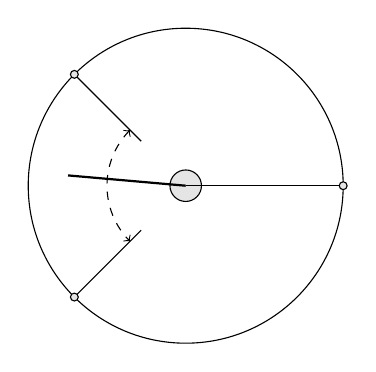
\begin{tikzpicture}
\pic {mechanicalSwitch};   
\end{tikzpicture}

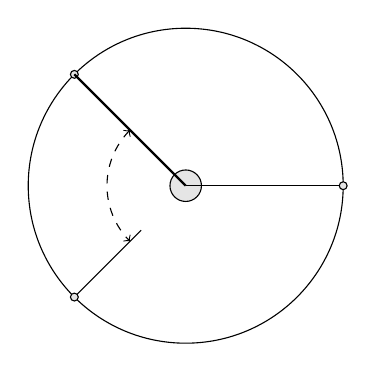
\begin{tikzpicture}
\pic {mechanicalSwitchClosed};   
\end{tikzpicture}



\begin{tikzpicture}
  \node [client] (a) {A}; 
  \node [client,below=1cm of a] (b) {B}; 
  \node [client,right=3cm of a] (c) {C}; 
  \node [client,right=3cm of b] (d) {D}; 

  \coordinate (tmp) at ([xshift=1cm,yshift=-0.5cm]a.east); 
  \coordinate (tmp2) at ([xshift=2cm,yshift=-0.5cm]a.east);
  \coordinate (center) at ($(a)!0.5!(d)$);

  \node [switch] (sw) at (center) {};
  \draw [thick] (a.east) -| (sw.135) (sw.225) |- (b.east); 
  \draw [thick] (c.west) -| (sw.45) (sw.315) |- (d.west); 
  % \draw [thick] (tmp)  -- (tmp2);

  \coordinate (tmp3) at ([yshift=-0.5cm]b.south);
  \node at (tmp3) {}; 
\end{tikzpicture}


% open switch 
\begin{tikzpicture}
  \node [client] (a) {A}; 
  \node [client,below=1cm of a] (b) {B}; 
  \node [client,right=3cm of a] (c) {C}; 
  \node [client,right=3cm of b] (d) {D}; 

  \coordinate (center) at ($(a)!0.5!(d)$);
  
  
  \coordinate (tmp) at ([xshift=-0.5cm]center); 
  \coordinate (tmp2) at ([xshift=0.5cm]center); 

  \node [switch, scale=2.5, ultra nearly transparent] (sw) at (center) {};

  
  \pic (ls) at (tmp) [scale=0.2] {mechanicalSwitch}; 
  \pic (rs) at  (tmp2) [rotate=180,scale=0.2] {mechanicalSwitch}; 

  \draw [thick] (a.east) -| (ls-inUp) (b.east) -| (ls-inDown);
  \draw [thick] (c.west) -| (rs-inDown) (d.west) -| (rs-inUp);
  \draw [thick] (ls-out) -- (rs-out); 
  

  
  % \draw [thick] (a.east) -| (sw.135) (sw.225) |- (b.east); 
  % \draw [thick] (c.west) -| (sw.45) (sw.315) |- (d.west); 
  % \draw [thick] (tmp)  -- (tmp2);

  % deal with the moeptikz bounding box bug
  \coordinate (tmp3) at ([yshift=-0.5cm]b.south);
  \node at (tmp3) {}; 
\end{tikzpicture}

% closed Switch 
\begin{tikzpicture}
  \node [client] (a) {A}; 
  \node [client,below=1cm of a] (b) {B}; 
  \node [client,right=3cm of a] (c) {C}; 
  \node [client,right=3cm of b] (d) {D}; 

  \coordinate (center) at ($(a)!0.5!(d)$);
  
  
  \coordinate (tmp) at ([xshift=-0.5cm]center); 
  \coordinate (tmp2) at ([xshift=0.5cm]center); 

  \node [switch, scale=2.5, ultra nearly transparent] (sw) at (center) {};

  
  \pic (ls) at (tmp) [scale=0.2] {mechanicalSwitchClosed}; 
  \pic (rs) at  (tmp2) [rotate=180,scale=0.2] {mechanicalSwitchClosed}; 

  \draw [thick] (a.east) -| (ls-inUp) (b.east) -| (ls-inDown);
  \draw [thick] (c.west) -| (rs-inDown) (d.west) -| (rs-inUp);
  \draw [thick] (ls-out) -- (rs-out); 
  
  
  % \draw [thick] (a.east) -| (sw.135) (sw.225) |- (b.east); 
  % \draw [thick] (c.west) -| (sw.45) (sw.315) |- (d.west); 
  % \draw [thick] (tmp)  -- (tmp2);

  % deal with the moeptikz bounding box bug
  \coordinate (tmp3) at ([yshift=-0.5cm]b.south);
  \node at (tmp3) {}; 


  \draw [very thick, hpired] (a.east) -- (a.east -| ls-inUp) -- (ls-inUp) -- (ls-center) -- (ls-out)-- (rs-out) -- (rs-center)-- (rs-inUp) -- (rs-inUp |- d.west) -- (d.west); 

%   \draw [very thick, hpiorange] plot [smooth, tension=1.5] coordinates {(a.east)  (ls-inUp) (ls-out) (rs-out)  (rs-inUp) (d.west)}; 
  
\end{tikzpicture}

\begin{tikzpicture}
  \draw [->] (0,0) -- (10,0);
  \draw [->] (0,0) -- (0, 5);

  \node [anchor=north west] at (10,0) {$t$}; 
  \node [anchor=east,align=center] at (0,5) {data\\rate}; 

  \draw [hpiblue, thick, dotted] (0, 1.3) node [anchor=east, align=center] {average\\rate} -- (10, 1.3);
  \draw [hpiorange, thick, dotted] (0, 4.9)  -- (10, 4.9)  node [anchor=south west, align=center]  {peak\\rate};

  \draw [hpired] plot [smooth] coordinates {(0,0.2) (1,0.5) (2,3.9) (3,4.7) (4, 0.3) (5, 0.4) (6, 0.2) (7, 4.2) (8, 0.9) (9, 4.5) (10, 2.3) };
  \node [anchor=west, align=center, hpired] at (10, 2) {Instantaneous\\rate};   
\end{tikzpicture}


% Packet switch, just with memory

\newcommand{\switchWithMemory}[0]{  \node [client, fill=hpired] (a) {A}; 
  \node [client,below=1cm of a, fill=hpiorange] (b) {B}; 
  \node [client,right=3cm of a, fill=hpiyellow] (c) {C}; 
  \node [client,right=3cm of b, fill=hpiblue] (d) {D}; 

  \coordinate (center) at ($(a)!0.5!(d)$);
  
  
  \coordinate (tmp) at ([xshift=-0.5cm]center); 
  \coordinate (tmp2) at ([xshift=0.5cm]center); 

  \node [switch, scale=2.5, ultra nearly transparent] (sw) at (center) {};

  % \node [ draw, anchor=north west, scale=0.5] (q_nw) at ([xshift=-5,yshift=5]sw.north west) { Buffer } ; 

  
  % \node [ draw, anchor=north east, scale=0.5] (q_ne) at ([xshift=5,yshift=5]sw.north east) { Buffer } ; 
  
  % \node [ draw, anchor=south east, scale=0.5] (q_se) at ([xshift=5,yshift=-5]sw.south east) { Buffer } ; 

  % \node [ draw, anchor=south west, scale=0.5] (q_sw) at ([xshift=-5,yshift=-5]sw.south west) { Buffer } ; 
  
  \node [fill=white, draw, minimum width=10, minimum height=10] at (center) (memory) {Memory}; 

  % do we put the interfaces at the switch border or the memory border? 
  
  \foreach \nn/\n/\e/\w in {ne/north east/c/west, nw/north west/a/east, sw/south west/b/east, se/south east/d/west} {
    \node [fill, circle, scale=0.2] (ifce_\nn) at (sw.\n) {};
    \draw [thick] (ifce_\nn) -- (\e.\w); 
    }
  
  % \foreach \n/\q/\w in {a.east/memory/north west, b.east/memory/south west, c.west/memory/north east, d.west/memory/south east} {
  %   % \node [fill, circle, scale=0.2] at (\q.\w)  {}; 
  %   \draw [very thick] (\n ) -- (\q.\w) node  [fill, circle, scale=0.3] {};
  %   % \draw (\q) -| (memory); 
  % }


  % and plenty of lines:
  
 
  
  % deal with the moeptikz bounding box bug
  \coordinate (tmp3) at ([yshift=-0.5cm]b.south);
  \node at (tmp3) {}; 
}

\begin{tikzpicture}
  \label{page:basics:switching:packet_just_memory}

  \switchWithMemory
\end{tikzpicture}



% Packet switch, with queue buffers 

\begin{tikzpicture}
  \label{page:basics:switching:packet_buffers}
  
  \node [client, fill=hpired] (a) {A}; 
  \node [client,below=1cm of a, fill=hpiorange] (b) {B}; 
  \node [client,right=3cm of a, fill=hpiyellow] (c) {C}; 
  \node [client,right=3cm of b, fill=hpiblue] (d) {D}; 

  \coordinate (center) at ($(a)!0.5!(d)$);
  
  
  \coordinate (tmp) at ([xshift=-0.5cm]center); 
  \coordinate (tmp2) at ([xshift=0.5cm]center); 

  \node [switch, scale=2.5, ultra nearly transparent] (sw) at (center) {};

  \node [ draw, anchor=north west, scale=0.5] (q_nw) at ([xshift=-5,yshift=5]sw.north west) { Buffer } ; 

  
  \node [ draw, anchor=north east, scale=0.5] (q_ne) at ([xshift=5,yshift=5]sw.north east) { Buffer } ; 
  
  \node [ draw, anchor=south east, scale=0.5] (q_se) at ([xshift=5,yshift=-5]sw.south east) { Buffer } ; 

  \node [ draw, anchor=south west, scale=0.5] (q_sw) at ([xshift=-5,yshift=-5]sw.south west) { Buffer } ; 
  
  \node [fill=white, draw] at (center) (memory) {Memory}; 

  \foreach \n/\q/\w in {a.east/q_nw/west, b.east/q_sw/west, c.west/q_ne/east, d.west/q_se/east} {
    \node [fill, circle, scale=0.2] at (\q.\w)  {}; 
    \draw [very thick] (\n |- \q) -- (\q);
    \draw (\q) -| (memory); 
  }


  % and plenty of lines:
  
 
  
  % deal with the moeptikz bounding box bug
  \coordinate (tmp3) at ([yshift=-0.5cm]b.south);
  \node at (tmp3) {}; 

\end{tikzpicture}


% Packet switch, with separate queues 

\begin{tikzpicture}
  \label{page:basics:switching:packet_in_out_queues}
  
  \node [client, fill=hpired] (a) {A}; 
  \node [client,below=1cm of a, fill=hpiorange] (b) {B}; 
  \node [client,right=3cm of a, fill=hpiyellow] (c) {C}; 
  \node [client,right=3cm of b, fill=hpiblue] (d) {D}; 

  \coordinate (center) at ($(a)!0.5!(d)$);
  
  
  \coordinate (tmp) at ([xshift=-0.5cm]center); 
  \coordinate (tmp2) at ([xshift=0.5cm]center); 

  \node [switch, scale=2.5, ultra nearly transparent] (sw) at (center) {};

  \node [rectangle split, rectangle split parts=6,
  rectangle split horizontal, text height=0.5cm,text depth=0.25cm,
  rectangle split part fill={white, hpiorange!20, hpiyellow!20, hpiyellow!20,hpiblue!20,hpiblue!20},
  draw, anchor=north west, scale=0.25] (q_nw_in) at ([xshift=-5,yshift=5]sw.north west) {  } ; 

  \node [rectangle split, rectangle split parts=6,
  rectangle split horizontal, text height=0.5cm,text depth=0.25cm,
  rectangle split part fill={  hpired!20,hpired!20,hpired!20, white, white, white,},
  draw, scale=0.25, above=0.1cm of q_nw_in] (q_nw_out)  {  } ; 

  \node [fill, circle, scale=0.2] (ifc_nw) at ([xshift=-2]$(q_nw_in.west)!0.5!(q_nw_out.west)$)  {}; 
  

  \node [rectangle split, rectangle split parts=6,
  rectangle split horizontal, text height=0.5cm,text depth=0.25cm,
  rectangle split part fill={hpiblue!20, hpired!20, hpiorange!20, hpiyellow!20, white, white,},
  draw, anchor=north east, scale=0.25] (q_ne_in) at ([xshift=5,yshift=5]sw.north east) {  } ; 

  \node [rectangle split, rectangle split parts=6,
  rectangle split horizontal, text height=0.5cm,text depth=0.25cm,
  rectangle split part fill={  white, white, white, white, white, hpiyellow!20, },
  draw, scale=0.25, above=0.1cm of q_ne_in] (q_ne_out)  { } ; 

  \node [fill, circle, scale=0.2] (ifc_ne) at ([xshift=2]$(q_ne_in.east)!0.5!(q_ne_out.east)$)  {}; 


  
  \node [rectangle split, rectangle split parts=6,
  rectangle split horizontal, text height=0.5cm,text depth=0.25cm,
  rectangle split part fill={hpired!20, hpiorange!20, hpired!20, hpiyellow!20, white, white, white},
  draw, anchor=south east, scale=0.25] (q_se_in) at ([xshift=5,yshift=-5]sw.south east) {  } ; 

  \node [rectangle split, rectangle split parts=6,
  rectangle split horizontal, text height=0.5cm,text depth=0.25cm,
  rectangle split part fill={  white, white, white, white, white, hpiblue!20, },
  draw, scale=0.25, above=0.1cm of q_se_in] (q_se_out)  { } ; 

  \node [fill, circle, scale=0.2] (ifc_se) at ([xshift=2]$(q_se_in.east)!0.5!(q_se_out.east)$)  {}; 


  
  \node [rectangle split, rectangle split parts=6,
  rectangle split horizontal, text height=0.5cm,text depth=0.25cm,
  rectangle split part fill={white, white, hpired!20, hpiyellow!20, hpired!20, hpiyellow!20},
  draw, anchor=south west, scale=0.25] (q_sw_in) at ([xshift=-5,yshift=-5]sw.south west) {  } ; 

  \node [rectangle split, rectangle split parts=6,
  rectangle split horizontal, text height=0.5cm,text depth=0.25cm,
  rectangle split part fill={ hpiorange!20, hpiorange!20,  white, white, white, white,  },
  draw, scale=0.25, above=0.1cm of q_sw_in] (q_sw_out)  { } ; 

  \node [fill, circle, scale=0.2] (ifc_sw) at ([xshift=-2]$(q_sw_in.west)!0.5!(q_sw_out.west)$)  {}; 

  
  \node [fill=white, draw] at (center) (memory) {Memory}; 


  % and plenty of lines:

  % ifcaces to queues: 
  \draw [very thick,] (a.east |- ifc_nw) -- (ifc_nw);
  \draw [->] (ifc_nw) |- (q_nw_in.west); 
  \draw [<-] (ifc_nw) |- (q_nw_out.west); 

  \draw [very thick,] (c.west |- ifc_ne) -- (ifc_ne);
  \draw [->] (ifc_ne) |- (q_ne_in.east); 
  \draw [<-] (ifc_ne) |- (q_ne_out.east); 

  \draw [very thick,] (b.east |- ifc_sw) -- (ifc_sw);
  \draw [->] (ifc_sw) |- (q_sw_in.west); 
  \draw [<-] (ifc_sw) |- (q_sw_out.west); 

  \draw [very thick,] (d.west |- ifc_se) -- (ifc_se);
  \draw [->] (ifc_se) |- (q_se_in.east); 
  \draw [<-] (ifc_se) |- (q_se_out.east);

  % and queues to/from memory
  % \draw (q_nw_in.east) -| ($(q_nw_in.east)!025!(q_ne_in.west)$ |- memory);
  \foreach \q in {q_nw_in.east, q_nw_out.east, q_ne_in.west, q_ne_out.west, q_sw_in.east, q_sw_out.east, q_se_in.west, q_se_out.west} \draw (\q) -| (memory); 
  
  

  
  % deal with the moeptikz bounding box bug
  \coordinate (tmp3) at ([yshift=-0.5cm]b.south);
  \node at (tmp3) {}; 

\end{tikzpicture}

\begin{tikzpicture}
  \label{page:basics:switching:packet_forwarding_1}

  \switchWithMemory

  % send a packet over first link

  \draw [hpired, very thick, ->] (a.east) to node[above] (num) {\CircledTop{1}} (ifce_nw);
  \node [messageclosed, right= 0.1cm of num, scale=0.5, fill=hpiblue!20]  {}; 

  \draw [hpired, thick, ->] (ifce_nw) to[out=30,in=90] (memory.north); 
  
\end{tikzpicture}

\begin{tikzpicture}
  \label{page:basics:switching:packet_forwarding_store}

  \switchWithMemory

  % send a packet over first link

  \node [messageclosed, left= 0.1cm of memory.east, scale=0.5, fill=hpiblue!20]  {}; 

  
\end{tikzpicture}

\begin{tikzpicture}
  \label{page:basics:switching:packet_forwarding_2}

  \switchWithMemory

  % send a packet over first link

  \draw [hpired, very thick, ->] (ifce_se) to node[above] (num) {\CircledTop{2}} (d.west); 

  \node [messageclosed, left= 0.1cm of num, scale=0.5, fill=hpiblue!20]  {}; 
  \draw [hpired, thick, ->] (memory.south) to[out=270,in=120] (ifce_se); 

\end{tikzpicture}


\begin{tikzpicture}
  \label{page:basics:multi_hop_packet}
  \node [client, fill=hpired] (a) {A}; 
  \node [client,below=2cm of a, fill=hpiorange] (b) {B}; 
  \node [client,right=5cm of a, fill=hpiyellow] (c) {C}; 
  \node [client,right=5cm of b, fill=hpiblue] (d) {D}; 

  \coordinate (sw1pos) at ($(a)!0.33!(d)$);
  \coordinate (sw2pos) at ($(a)!0.66!(d)$);

  \node [switch] (sw1) at (sw1pos) {}; 
  \node [switch] (sw2) at (sw2pos) {}; 


  \draw [thick] (a.east) -- (sw1) -- (b.east) (sw1) --(sw2) -- (c.west) (sw2) -- (d.west);

  \draw [hpired, thick, ->]
  (a.east) edge [out=0, in=110] node [above] {\Circled{1}} (sw1.110)
  (sw1) edge [out=0, in=110] node [above] {\Circled{2}} (sw2)
  (sw2) edge [out=10, in=110] node [above] {\Circled{3}} (d.west)
  ; 
   

  % deal with the moeptikz bounding box bug
  \coordinate (tmp3) at ([yshift=-0.5cm]b.south);
  \node at (tmp3) {}; 
  
\end{tikzpicture}


\begin{tikzpicture}
  \label{fig:basics:msc:packet:multihop}

  \node [client, scale=0.5] at (0,0) (a) {A}; 
  \node [switch, scale=0.5] at (1,0) (sw1) {SW 1}; 
  \node [switch, scale=0.5] at (2,0) (sw2) {SW 2}; 
  \node [client, scale=0.5] at (3,0) (d) {D};

  \foreach \n in {a, sw1, sw2, d} \draw (\n) -- ++ (0, -10);

  
  
\end{tikzpicture}


\end{document}